\documentclass[12pt]{article}
\usepackage{graphicx}
\usepackage[margin=30mm, paper = a4paper]{geometry}
\usepackage{minted, caption}
\usepackage{subcaption}
\usepackage{multicol}

\title{}
\author{}
\date{}
\setlength{\columnseprule}{1pt}
\setlength{\columnsep}{2cm}
\begin{document}
\vspace*{\fill}
\begin{center}

    \emph{Heaven's Light is Our Guide} \\
    \textbf{Rajshahi University of Engineering and Technology} \\

    \begin{figure}[h]
        \centering
        
\includegraphics[scale=.34]{images/RUET_logo.png}
        \label{fig:ruet_logo}
    \end{figure}
    \vspace{5mm}

    \textbf{Course Code}\\
    ECE 2216\\
    \vspace{3mm}
    \textbf{Course Title}\\
    Database Systems Sessional

    \vspace{5mm}
    \textbf{Experiment Date:} October 15, 2023,\\
    \textbf{Submission Date:} November 5, 2023\\

    \vspace{5mm}
    \textbf{Lab Report 3:} Creating a database and doing operations on it using SQL\\

    \vspace{15mm}

    \begin{tabular}{c|c}
        \textbf{Submitted to} & \textbf{Submitted by} \\
        Md. Robiul Islam      & Md. Tajim An Noor     \\
        Assistant Professor   & Roll: 2010025         \\
        Dept of ECE, Ruet     &                       \\
    \end{tabular}

\end{center}
\vspace*{\fill}

\pagebreak

\tableofcontents

\maketitle

\section{Tools Used}
\begin{itemize}
    \item MySQL
    \item VS Code - as an IDE to use SQL
    \item MacTeX -\LaTeX  compiler
    \item VS Code with LaTeX workshop extension as a text editor
\end{itemize}


\section{Process}

\subsection*{SQL Codes:}
\subsubsection{Display the order number, order date \& the purchase amount for order(s) which will be delivered by the salesman with ID 5001.}
\subsubsection*{Code:}
\begin{minted}[breaklines, linenos]{mysql}
SELECT
    order_no as "Order No",
    order_date as "Order Date",
    purchase_amount as "Purchase Amount"
FROM
    Relations.Order
WHERE
    salesman_id = 5001
\end{minted}
\vspace{10mm}

\subsubsection{Find the customer name \& price of the cheapest items(s) using subquery.}
\subsubsection*{Code: }
\begin{minted}[breaklines, linenos]{mysql}
SELECT
    c.customer_name as "Customer Name",
    o.purchase_amount as "Purchase Amount"
from
    Relations.Customer c,
    Relations.Order o
WHERE
    c.customer_id = (
        SELECT
            customer_id
        FROM
            Relations.Order o
        WHERE
            purchase_amount = (
                SELECT
                    min(purchase_amount)
                FROM
                    Relations.Order
            )
    )
    AND purchase_amount = (
        SELECT
            min(purchase_amount)
        FROM
            Relations.Order
    )
\end{minted}

\vspace{10mm}

\subsubsection{Find those salesmen with all information who gets the commission within a range of 0.12 \& 0.14.}
\subsubsection*{Code: }
\begin{minted}[breaklines, breakanywhere, linenos]{mysql}
SELECT
    salesman_id as "Salesman ID",
    name as "Salesman Name",
    city as "City",
    commission as "Commission"
FROM
    Relations.salesman
WHERE
    commission >= 0.12
    AND commission <= 0.14
\end{minted}
\vspace{10mm}

\subsubsection{Find the total purchase amount of all orders.}
\subsubsection*{Code: }
\begin{minted}[breaklines, breakanywhere, linenos]{mysql}
SELECT
    sum(purchase_amount) as "Total Purchased Amount"
FROM
    Relations.Order
\end{minted}
\vspace{10mm}

\subsubsection{Find the highest purchase amount on date “2016-08-17” for each salesman with their ID.}
\subsubsection*{Code:}
\begin{minted}[linenos,breaklines,breakanywhere]{mysql}
SELECT
    MAX(purchase_amount) as "Max Purchased Amount",
    salesman_id as "Salesman ID",
    order_date as "Order Date"
FROM
    Relations.Order
WHERE
    order_date = "2016-08-17"
GROUP BY
    salesman_id
\end{minted}

\vspace{5mm}
\subsubsection{Display all the orders issued by the salesman “Paul Adam” from the orders table.}
\subsubsection*{Code:}
\begin{minted}[linenos,breaklines,breakanywhere]{mysql}
SELECT
    order_no as "Order No",
    purchase_amount as "Purchase Amount",
    order_date as "Order Date",
    customer_id as "Customer ID",
    salesman_id as "Salesman ID"
FROM
    Relations.Order
WHERE
    salesman_id = (
        SELECT
            salesman_id
        from
            Relations.salesman
        WHERE
            name = 'Paul Adam'
    )
\end{minted}

\section{Output}
\captionsetup{justification=centering}
\begin{figure}[htbp!]
    \begin{subfigure}{1\textwidth}
        \centering
        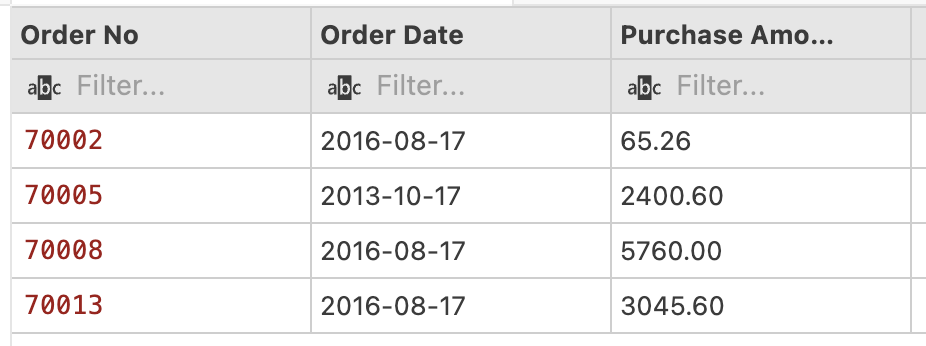
\includegraphics[width=\linewidth]{images/output/q1.png}
        \caption*{The person who is the top of the organization (i.e. reports to no one)}
        \label{fig:q1}
    \end{subfigure}
    \vspace*{20mm}
    \begin{subfigure}{.3\textwidth}
        \centering
        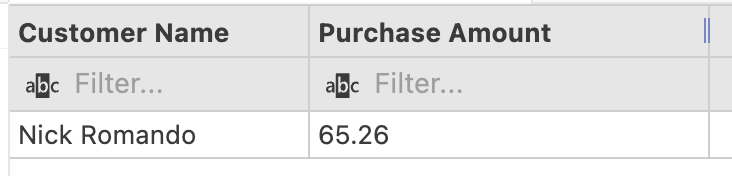
\includegraphics[width=.6\linewidth]{images/output/q2.png}
        \caption*{Difference in days between the most recent and oldest order date in Orders file.}
        \label{fig:q2}
    \end{subfigure}
    \begin{subfigure}{.3\textwidth}
        \centering
        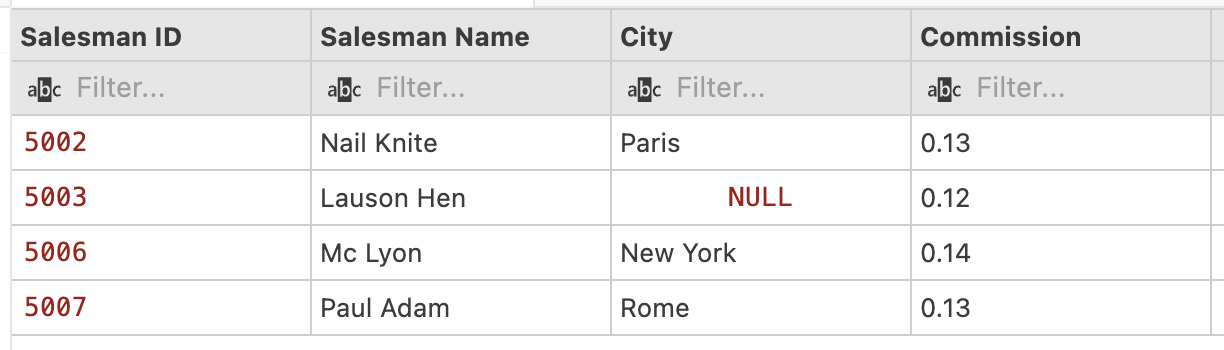
\includegraphics[width=.6\linewidth]{images/output/q3.png}
        \caption*{Total value of  payments received in July 2004.}
        \label{fig:q3}
    \end{subfigure}
    \begin{subfigure}{.3\textwidth}
        \centering
        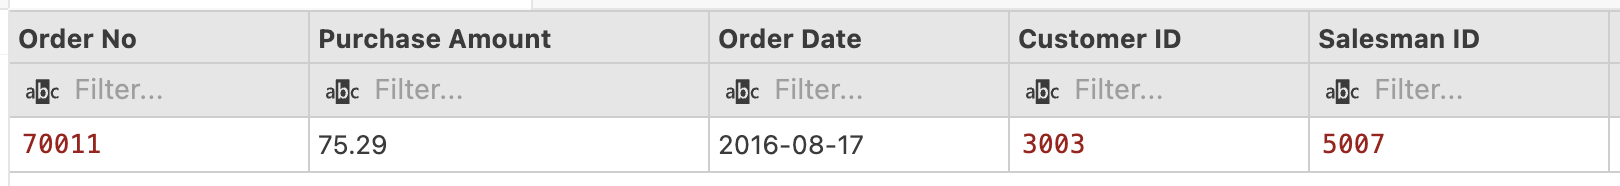
\includegraphics[width=.6\linewidth]{images/output/q6.png}
        \caption*{The number of orders ‘On Hold’ for each customer.}
        \label{fig:q6}
    \end{subfigure}

    \begin{subfigure}{\textwidth}
        \centering
        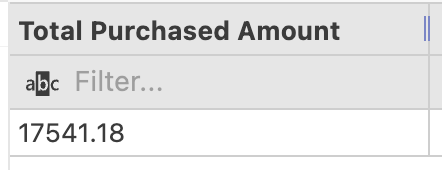
\includegraphics[width=.5\linewidth]{images/output/q4.png}
        \caption*{Profit generated by each sales representative based on the orders from the customers they serve. Sorted by profit generated descending.}
        \label{fig:q4}
    \end{subfigure}
    \begin{subfigure}{.5\textwidth}
        \centering
        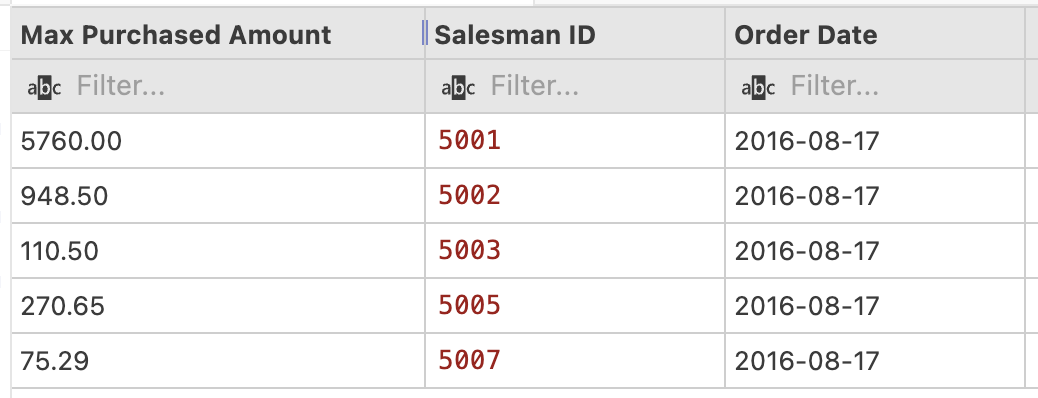
\includegraphics[width=.8\linewidth]{images/output/q5.png}
        \caption*{Products sold in 2003 but not 2004.}
        \label{fig:q5}
    \end{subfigure}
    \begin{subfigure}{.5\textwidth}
        \centering
        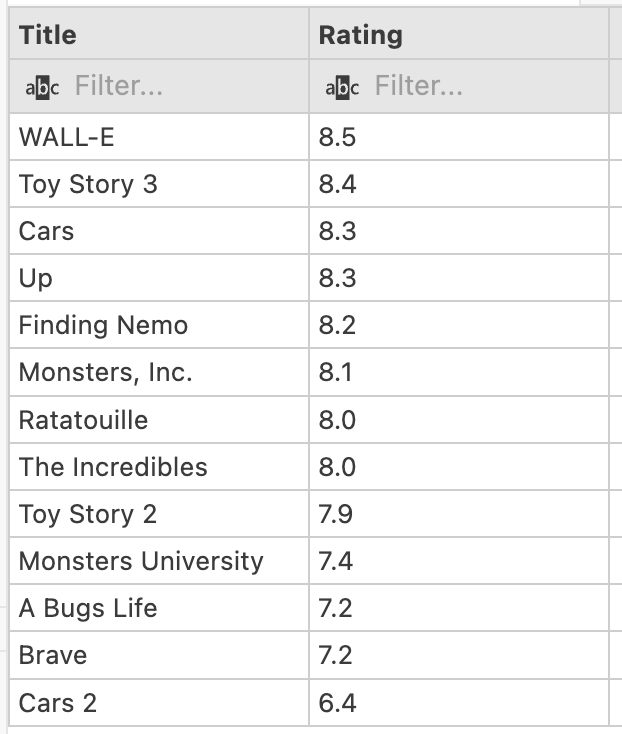
\includegraphics[width=.65\linewidth]{images/output/q7.png}
        \caption*{Names of products sold at less than 80\% of the MSRP.}
        \label{fig:q7}
    \end{subfigure}
\end{figure}

\end{document}